\documentclass{article}

\title{Scoary manual\\Version 1.6.12}

\date{}

\author{Ola Brynildsrud\\olbb@fhi.no}


\usepackage{graphicx}
\usepackage{listings}
\usepackage{tabularx}
\usepackage{booktabs}
\usepackage{ltxtable}

\lstset{
  basicstyle=\ttfamily,
  columns=fullflexible,
  frame=single,
  breaklines=true,
  % postbreak=\mbox{\textcolor{red}{$\hookrightarrow$}\space},
}

\begin{document}

  \pagenumbering{gobble}

  \maketitle

  \newpage

  \tableofcontents

  \newpage

  \pagenumbering{arabic}

  \begin{figure}
    
\includegraphics[width=\linewidth]{images/scoary_logo.png}
  \end{figure}

  \section{Scoary utility}

  Scoary \cite{brynildsrud2016rapid} is designed to take the gene\textunderscore presence\textunderscore absence.csv file from \textbf{Roary} \cite{page2015roary} as well as a traits file created by the user and calculate the assocations between all genes in the accessory genome and the traits. It reports a list of genes sorted by strength of association per trait.

  \section{Installation}

    \subsection{Dependencies}

    \begin{itemize}

      \item Python (Tested with versions 2.7, 3.4, 3.5, 3.6 and 3.6-dev)
      \item SciPy (Tested with versions 0.16, 0.17, 0.18)

    \end{itemize}

    \noindent If you supply custom trees (Optional)

    \begin{itemize}

      \item ete3
      \item six

    \end{itemize}

    \noindent Note that ete3 and six are not automatically installed. To get them use 
    \begin{lstlisting}[language=python, basicstyle=\small]
      $ pip install ete3 six
    \end{lstlisting}

    \noindent Using the GUI (Optional)

    \begin{itemize}

      \item Tkinter/ttk

    \end{itemize}

    \noindent Tkinter/ttk is already part of most python distributions. If you lack it consider getting Homebrew/Linuxbrew and then run
    \begin{lstlisting}[language=python, basicstyle=\small]
      $ brew install python --with-tcl-tk
    \end{lstlisting}

    \subsection{Installation}

    The easiest way to install Scoary is with the pip package manager:
    \begin{lstlisting}[language=python, basicstyle=\small]
      $ pip install scoary
    \end{lstlisting} 
    OR, if you need a local (user) installation:
    \begin{lstlisting}[language=python, basicstyle=\small]
      $ pip install --user scoary
    \end{lstlisting}
  \section{Basic usage}

    \subsection{Getting started}
      Basic command line:
      \begin{lstlisting}[language=python, basicstyle=\small]
        $ scoary -g gene_presence_absence.csv -t traits.csv
      \end{lstlisting}
    
      \noindent \textbf{Using the GUI} \\
      \noindent Those allergic to command line usage might want to use
      \begin{lstlisting}[language=python, basicstyle=\small]
        $ scoary_GUI
      \end{lstlisting}

      \noindent to bring up a graphical interface. It is fairly intuitive, has a progress bar and can show you an example. Note that if you use the GUI Scoary will be much slower than usual (especially of you are doing lots of permutations), so it is not recommended for users that are proficient in command line usage.

      \begin{figure}
        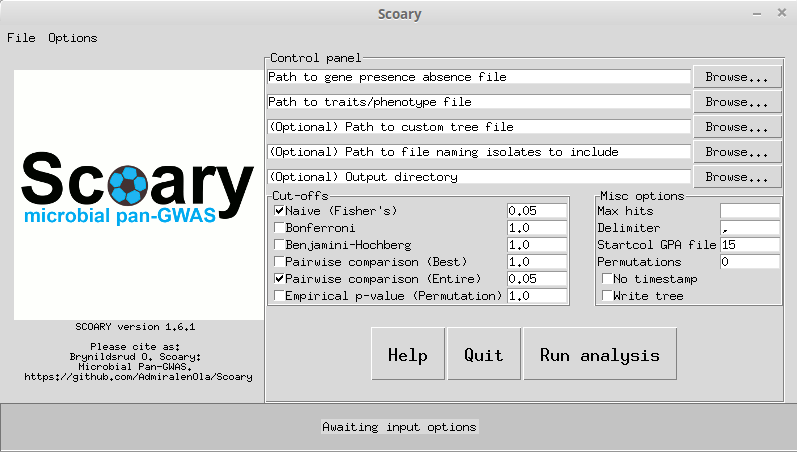
\includegraphics[width=\linewidth]{images/scoary_gui.png}
        \caption{Scoary GUI}
        \label{fig:gui}
      \end{figure}
    
    \subsection{Input}
      Scoary requires two input files: The gene\textunderscore presence\textunderscore absence.csv file from \textbf{Roary} and a list of traits to test associations to. Traits can be anything as long as you can classify it into binary categories. (e.g. antibiotic resistance, group membership (yes/no), MIC value higher/lower than 16). \\

      You can see an example of how the input files could look in the exampledata folder.
      \subsubsection{Gene presence/absence file}
        The gene\textunderscore presence\textunderscore absence.csv file will look something like this:
        \begin{figure}[h!]
        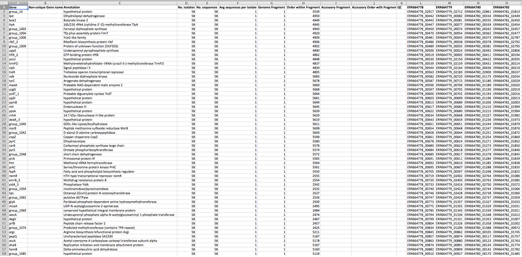
\includegraphics[width=\linewidth]{images/gene_presence_and_absence.png}
        \caption{Input Roary file (Source: http://sanger-pathogens.github.io/Roary)}
        \label{fig:gpa}
        \end{figure}

        \noindent Make sure you know the delimiter in the file. (By default this is ','). Scoary needs to know.\\

        \textbf{LS-BSR input}\\
        You can also use as input the pan-genome as called from Jason Sahl's program LS-BSR (Large-Scale Blast Score Ratio). The program includes a python script for converting LS-BSR output to the Roary/Scoary format.

      \subsubsection{Traits file}
        The \textbf{traits.csv} file needs to be formatted in a specific way.
        \begin{itemize}
          \item It must use the same delimiter as the gene\textunderscore presence\textunderscore absence.csv file
          \item The names of your isolates need to be identical in the two files
          \item The rows should correspond to your isolates, the columns to the different traits
          \item Traits needs to be dichotomized. Use "0" to indicate absence and "1" to indicate presence of the trait
          \item All isolates and traits should be uniquely named and not contain any weird characters (e.g. \& \% \$ \# \_ \{ \} @ ? etc)
          \item The top left cell should be left blank
        \end{itemize}
        \noindent It should look something like this: \\

        \LTXtable{\textwidth}{tables/t1.tex}

        \textbf{Missing data} \\
        Don't worry if you have not measured the phenotype for all your traits. From v1.6.9 on, Scoary can handle missing data. The missing values need to be specified as "NA", "." or "-". Note that Scoary does not actually specify any kind of uncertainty model for these missing values, it simply excludes them from further analysis. \\
    
      \subsubsection{Converting VCF files to use as Scoary input}
        From version 1.6.12, Scoary has a function for converting VCF files to the Roary/Scoary format. This allows you to use a wide range of variants (e.g SNPs, indels, structural variants etc) in your input.\\

        The script can be run using the following command:
        \begin{lstlisting}[language=python, basicstyle=\small]
          $ vcf2scoary myvariants.vcf
        \end{lstlisting}

        The current vcf2scoary script is a beta version, and may not correctly handle every VCF file. (Please report bugs!) \\

        Note that Scoary simplifies analysis for variants with more than 2 alleles. Rather than comparing all possible contrasts, it compares each non-reference with the reference. Say for example that 4 different alleles exist at a known SNP site. Let's call them A, C, G, and T, and let A be the reference allele. (The reference category is always inferred from the VCF file). This allele can be encoded in a single line in a VCF file, but in the Scoary format it needs to be spread over 3 different lines. (One for each contrast to the reference, i.e. A vs C, A vs G, and A vs T). Thus, not every possible contrast is tested in the association analysis! It is for example possible that there is a real difference in phenotype between G and T, but this contrast is not tested.
    
    \subsection{Output}
      Scory outputs a single csv file per trait in the traits file. It uses comma "," as a delimiter. The results consists of genes that were found to be associated with the trait, sorted according to significance. (By default, Scoary reports all genes with a naive p-value $< 0.05$, but the user can change the cut-off value and use adjusted p-values instead) \\

      An explanation of the different columns in the output can be seen in Table \ref{tab:cols}: \\
      
      \LTXtable{\textwidth}{tables/t2.tex}

  \section{Advanced usage}
    Scoary can take a number of optional arguments to tweak the output and make sure it performs as intended:
    \begin{lstlisting}[basicstyle=\fontsize{6}{11}\ttfamily,breaklines]
      $ scoary -h
      usage: scoary.py [-h] [-t TRAITS] [-g GENES] [-o OUTDIR]
                       [-p P_VALUE_CUTOFF [P_VALUE_CUTOFF ...]]
                       [-c [{I,B,BH,PW,EPW,P} [{I,B,BH,PW,EPW,P} ...]]] [-e PERMUTE]
                       [-m MAX_HITS] [-r RESTRICT_TO] [-w] [-s START_COL] [-u]
                       [-n NEWICKTREE] [--delimiter DELIMITER] [--collapse]
                       [--threads THREADS] [--no-time] [--test] [--citation]
                       [--version]

      Scoary version 1.6.10 - Screen pan-genome for trait-associated genes

      optional arguments:
        -h, --help            show this help message and exit
        -t TRAITS, --traits TRAITS
                              Input trait table (comma-separated-values). Trait
                              presence is indicated by 1, trait absence by 0.
                              Assumes strain names in the first column and trait
                              names in the first row
        -g GENES, --genes GENES
                              Input gene presence/absence table (comma-separated-
                              values) from ROARY. Strain names must be equal to
                              those in the trait table
        -o OUTDIR, --outdir OUTDIR
                              Directory to place output files. Default = .
        -p P_VALUE_CUTOFF [P_VALUE_CUTOFF ...], --p_value_cutoff P_VALUE_CUTOFF [P_VALUE_CUTOFF ...]
                              P-value cut-off / alpha level. For Fishers,
                              Bonferronis, and Benjamini-Hochbergs tests, SCOARY
                              will not report genes with higher p-values than this.
                              For empirical p-values, this is treated as an alpha
                              level instead. I.e. 0.02 will filter all genes except
                              the lower and upper percentile from this test. Run
                              with "-p 1.0" to report all genes. Accepts standard
                              form (e.g. 1E-8). Provide a single value (applied to
                              all) or exactly as many values as correction criteria
                              and in corresponding order. (See example under
                              correction). Default = 0.05
        -c [{I,B,BH,PW,EPW,P} [{I,B,BH,PW,EPW,P} ...]], --correction [{I,B,BH,PW,EPW,P} [{I,B,BH,PW,EPW,P} ...]]
                              Apply the indicated filtration measure. I=Individual
                              (naive) p-value. B=Bonferroni adjusted p-value. BH
                              =Benjamini-Hochberg adjusted p. PW=Best (lowest)
                              pairwise comparison. EPW=Entire range of pairwise
                              comparison p-values. P=Empirical p-value from
                              permutations. You can enter as many correction
                              criteria as you would like. These will be associated
                              with the p_value_cutoffs you enter. For example "-c I
                              EPW -p 0.1 0.05" will apply the following cutoffs:
                              Naive p-value must be lower than 0.1 AND the entire
                              range of pairwise comparison values are below 0.05 for
                              this gene. Note that the empirical p-values should be
                              interpreted at both tails. Therefore, running "-c P -p
                              0.05" will apply an alpha of 0.05 to the empirical
                              (permuted) p-values, i.e. it will filter everything
                              except the upper and lower 2.5 percent of the
                              distribution. Default = Individual p-value. (I)
        -e PERMUTE, --permute PERMUTE
                              Perform N number of permutations of the significant
                              results post-analysis. Each permutation will do a
                              label switching of the phenotype and a new p-value is
                              calculated according to this new dataset. After all N
                              permutations are completed, the results are ordered in
                              ascending order, and the percentile of the original
                              result in the permuted p-value distribution is
                              reported.
        -m MAX_HITS, --max_hits MAX_HITS
                              Maximum number of hits to report. SCOARY will only
                              report the top max_hits results per trait
        -r RESTRICT_TO, --restrict_to RESTRICT_TO
                              Use if you only want to analyze a subset of your
                              strains. Scoary will read the provided comma-separated
                              table of strains and restrict analyzes to these.
        -w, --write_reduced   Use with -r if you want Scoary to create a new gene
                              presence absence file from your reduced set of
                              isolates. Note: Columns 1-14 (No. sequences, Avg group
                              size nuc etc) in this file do not reflect the reduced
                              dataset. These are taken from the full dataset.
        -s START_COL, --start_col START_COL
                              On which column in the gene presence/absence file do
                              individual strain info start. Default=15. (1-based
                              indexing)
        -u, --upgma_tree      This flag will cause Scoary to write the calculated
                              UPGMA tree to a newick file
        -n NEWICKTREE, --newicktree NEWICKTREE
                              Supply a custom tree (Newick format) for phylogenetic
                              analyses instead instead of calculating it internally.
        --delimiter DELIMITER
                              The delimiter between cells in the gene
                              presence/absence and trait files, as well as the
                              output file.
        --collapse            Add this to collapse correlated genes (genes that have
                              identical distribution patterns in the sample) into
                              merged units.
        --threads THREADS     Number of threads to use. Default = 1
        --no-time             Output file in the form TRAIT.results.csv, instead of
                              TRAIT_TIMESTAMP.csv. When used with the -w argument
                              will output a reduced gene matrix in the form
                              gene_presence_absence_reduced.csv rather than
                              gene_presence_absence_reduced_TIMESTAMP.csv
        --test                Run Scoary on the test set in exampledata, overriding
                              all other parameters.
        --citation            Show citation information, and exit.
        --version             Display Scoary version, and exit.

      by Ola Brynildsrud (olbb@fhi.no)
    \end{lstlisting}

    \subsection{Restricting analysis to a subset of isolates with the -r parameter}
      The \textbf{-r} parameter is particularly useful, as you can use it to restrict your analysis to a subset of your isolates without altering the gene\textunderscore presence\textunderscore absence or trait files. Simply provide a single-line csv file (delimited by ",") with the names of the isolates you would like to include in the current analysis.\\

      This can be useful for example if you have multiple clades in your dataset but would like to restrict analysis to just one clade. Maybe the trait determinant is not the same in the two clades? Or perhaps you have missing data for some isolates?\\

      The provided file can look something like this:\\

      \begin{lstlisting}[language=bash]
        Strain1,Strain2,Strain4,Strain9
      \end{lstlisting}

      This will restrict the current analysis to isolates 1, 2, 4 and 9, and will omit all others.\\

      \textbf{Writing a reduced representation input file with the -w flag}\\

      Using the \textbf{-w} flag with \textbf{-r} will make Scoary write a reduced gene presence/absence file containing only those isolates specified with \textbf{-r}. This makes the program run much faster if you are analyzing a small subset of a large dataset.\\

    \subsection{Getting input right when using non-standard Roary files using -s}

      The \textbf{-s} parameter is used to indicate to Scoary which column in the \\ gene\textunderscore presence\textunderscore absence.csv file is the \textit{first} column representing an isolate. By default it is set to 15 (1-based indexing).

    \subsection{Controlling the output}
    
      The -p, -m and -c parameters further control your output. \textbf{-m} sets a hard cut-off on the number of hits reported. With \textbf{-p} you can set that no gene with a higher p-value will be reported. (Tip: Set this to 1.0 to report every single gene). \textbf{-c} specifies which cutoffs this threshold should apply to. For example, if you only wanted genes with a Bonferroni-adjusted p-value $< 1E-10$ you could use -p 1E-10 -c B. \\

      You can also mix different restrictions together. For example, you may want to specify that the entire range of pairwise comparisons p-values be $< 1E-5$, but you still doubt some of your results. You could try to filter your results more strictly by also requiring an Individual (naive) p-value of less than 0.01. You would then use -c EPW I -p 1E-5 0.01. You need to enter the -c options and the -p options in the corresponding order. \\

      Alternatively, you can specify a single (one) p-value, and this will be taken as the filter for all the specified -c options. For example -c EPW BH -p 0.05 will filter the results to only include genes where the entire range of pairwise comparison as well as the Benjamini-Hochberg p-values are $> 0.05$ \\

    \subsection{Writing a newick tree}
      Calling Scoary with the \textbf{-u} flag will cause it to write a newick file of the UPGMA tree that is calculated internally. The tree is based on pairwise Hamming distances in the gene\textunderscore presence\textunderscore absence matrix. Taxa have to be named the same as they are in the gene presence/absence and trait files. \\

    \subsection{Setting a custom tree with the -n parameter}
      You can (in fact you should) supply a custom phylogenetic tree (in newick format) to Scoary. This tree will be used for calculating contrasting pairs rather than Scoary using the Hamming distances in the gene presence absence file for UPGMA calculation. \\

      Note: The input sample tree topology is a fixed parameter in Scoary. It is assumed to be without error. By default, Scoary calculates a UPGMA tree topology internally from the presence/absence status in the gene presence/absence matrix, which is probably not the most robust data for phylogenetic inference. Since pairwise comparisons rely on the branching order in the tree, a best practices approach would be to supply tree(s) that you have calculated using a more robust approach (e.g. a ML tree based on your sequence data).\\

      \textbf{Recombination}\\
      Although some bacteria evolve clonally, most have very reticulate evolutionary histories as a result of recombination. Scoary population structure handling is built for tree-like evolution. It is therefore recommended that you supply to Scoary a tree where putative recombination has been excluded. Some popular options to create such trees are Gubbins, ClonalFrameML and BRATNextGen. \\

    \subsection{Post-analysis label-switching permutations}
      Use \textbf{-e X} to permute the dataset X times, rank the test estimators (number of successes (AB-ab pairs) / total number of contrasting pairs (ie. AB-ab and Ab-aB)) and report the unpermuted test estimator's empirical p-value. Calculated as $(r+1)/(n+1)$ where r is the number of estimators that exceed the unpermuted estimator in value and n is the total number of permutations \cite{north2002note}. Empirical p-values are great for deciding if your result looks significant just by coincidence or by a true association. The permutation procedure destroys the relationship between the variant and the phenotype, making the null hypothesis true. Each permutation test estimator is sampled under the null hypothesis. If these data look like your real data, you're in trouble. So if your empirical p-value is not low, chances are you seeing a false positive results even if your other p-values (Bonferroni, pairwise comparisons etc) indicate significance of the variant. You can use empirical p-values as a results filter by using \textbf{-c P}.\\

    \subsection{Collapsing correlated variants}
      Adding the \textbf{--collapse} flag to the command line will collapse genes that are identically distributed in your sample. For example, plasmid genes are often inherited together and as such will not add any information individually. From a statistical point of view, this is more correct, as in the opposite case the program will test (and correct for) multiple identical null hypotheses, thus unfairly penalizing your results by multiple comparisons correction. \\

  \section{Population structure}
    Scoary implements the pairwise comparisons algorithm \cite{read1995inference,maddison2000testing} to identify the maximum number of non-intersecting pairs of isolates that contrast in the state of both gene and trait. It does this by creating an UPGMA tree from the information contained in the gene\textunderscore presence\textunderscore absence matrix, annotating tips with gene and trait status, and recursively traversing the tree for each gene that were significant in the initial analysis. (i.e. those with $p<0.05$ if settings are left at default.) \\

    This tells you something about the \textit{number of times} the gene and trait co-emerged in the evolutionary history of your sample. Consider the trees in Figure \ref{fig:badlink} and in Figure \ref{fig:goodlink}. In both scenarios, the gene perfectly predict the trait status, with 10 positive and 11 negative isolates, corresponding to a naïve p-value of 2.8E-6. However, in the tree in Figure \ref{fig:badlink}, there is a maximum of two non-intersecting contrasting pairs, which must be considered relatively weak evidence for a causal link between this gene and the trait. There can be many other evolutionary events at the stars that explain the observed distribution equally well as this gene. In the tree in Figure \ref{fig:goodlink}, however, there is a maximum of seven possible non-intersecting contrasting pairs, which implies that this gene and the trait co-emerged seven times. This would be considered far stronger evidence for a causal link between the gene and the trait. \\

    \begin{figure}
      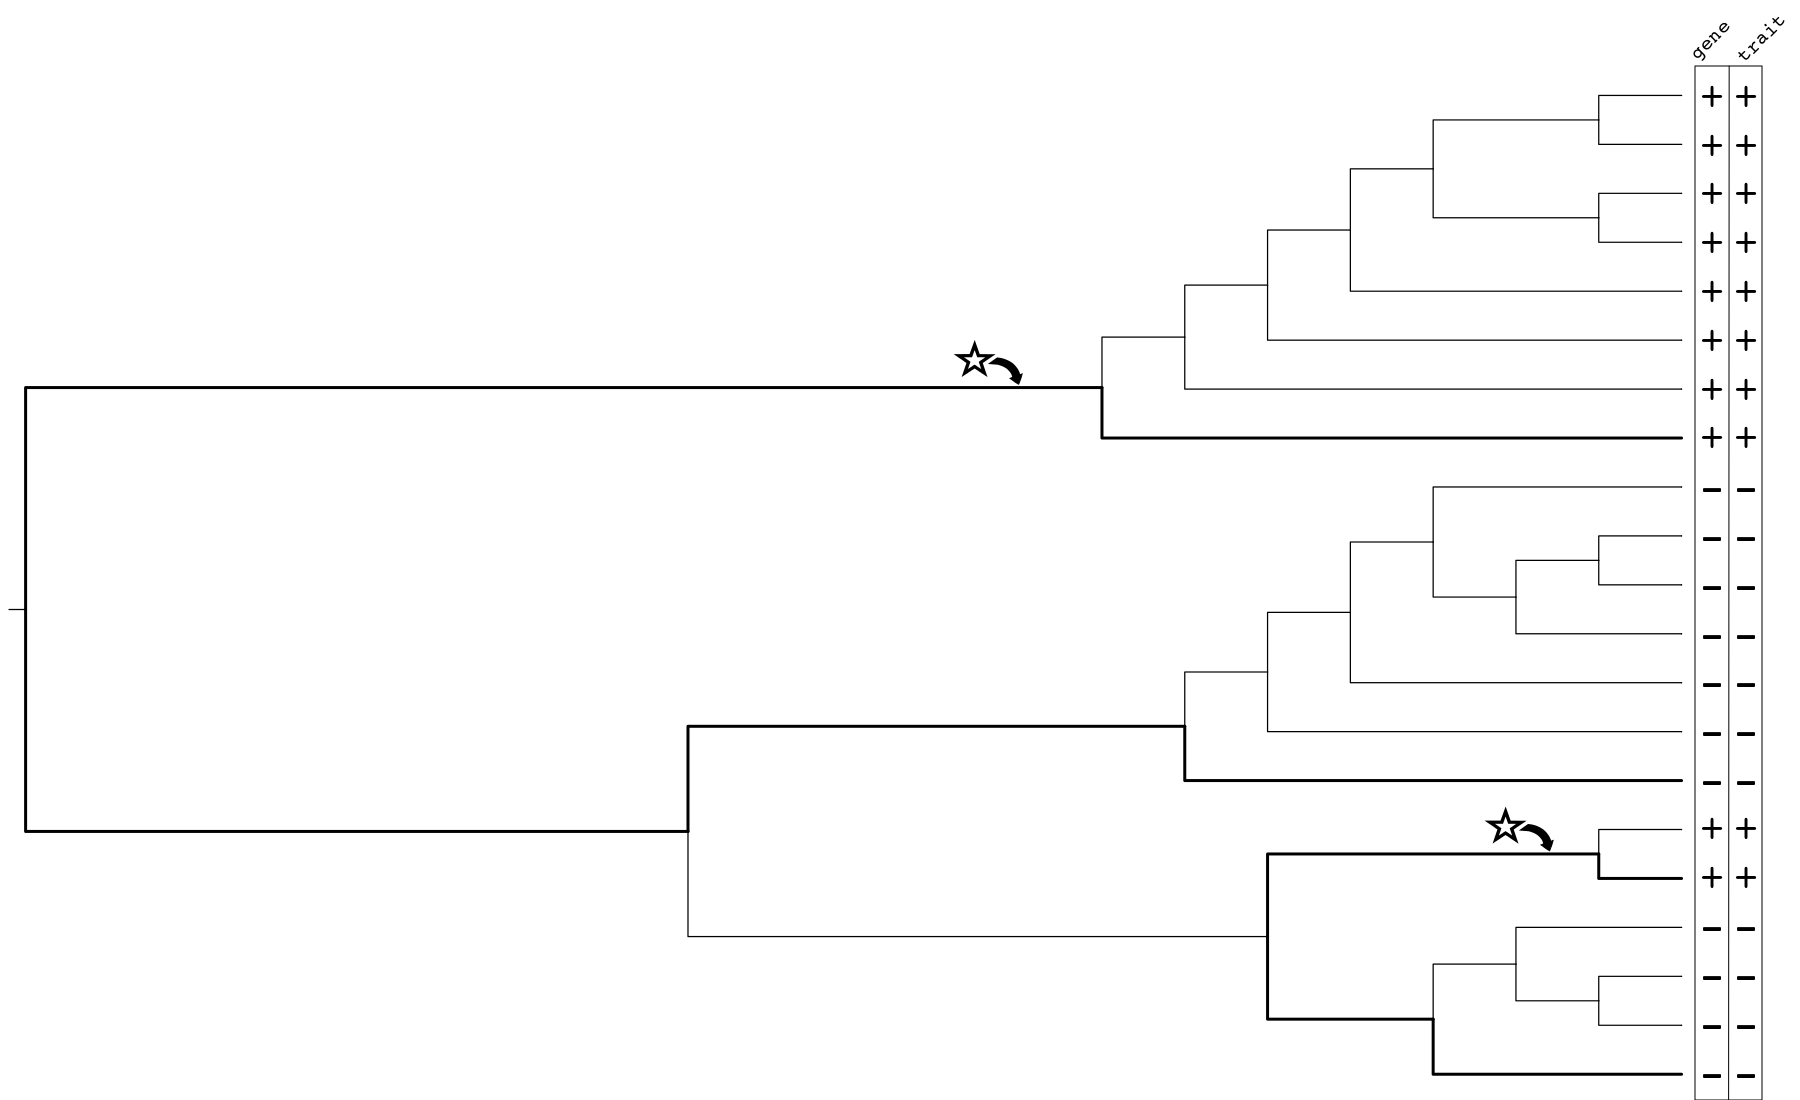
\includegraphics[width=\linewidth]{images/badlink.png}
      \caption{A not-so-significant link between gene and trait}
      \label{fig:badlink}
    \end{figure}

    \begin{figure}
      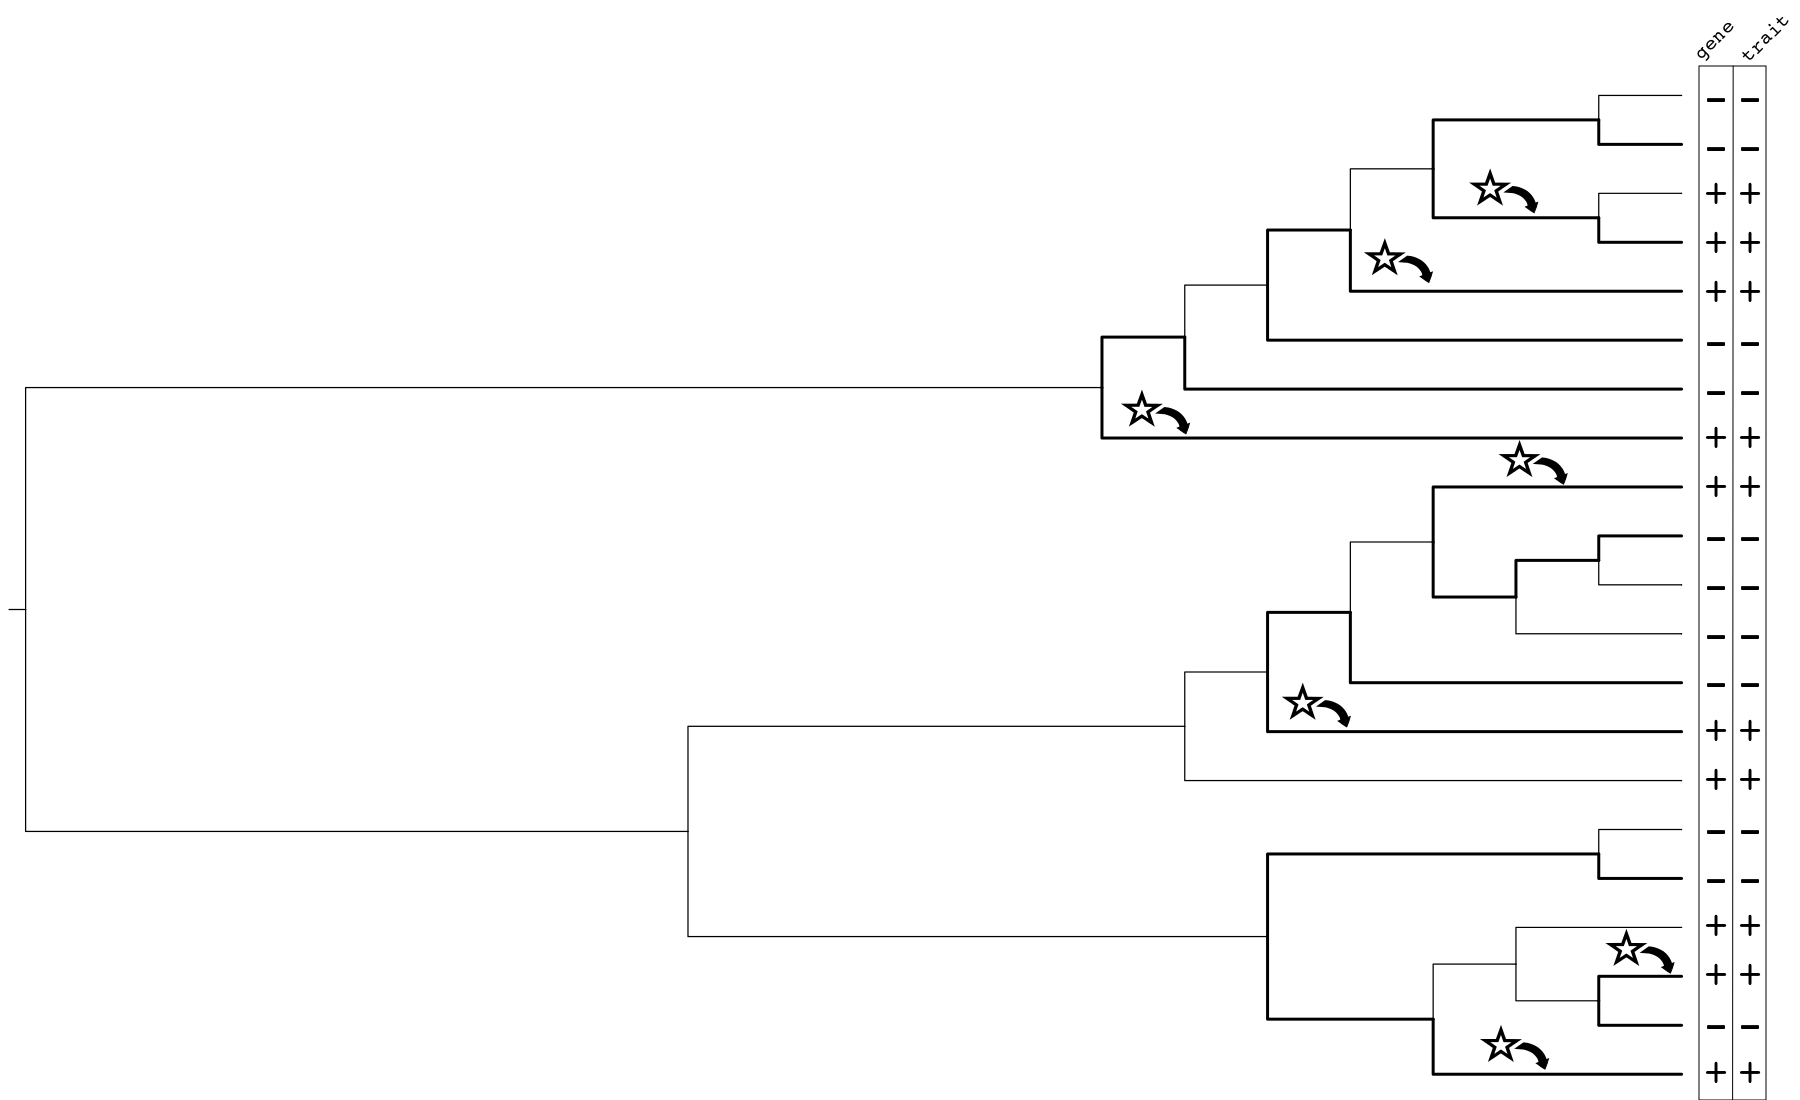
\includegraphics[width=\linewidth]{images/goodlink.png}
      \caption{A significant link between gene and trait}
      \label{fig:goodlink}
    \end{figure}

    One must also consider that there might be multiple ways of picking the maximum number of contrasting pairs, and of all these possible sets of pairings, some might provide more support for \verb+A->B+ than others. Consider the tree in Figure \ref{fig:best}: \\

    \begin{figure}
      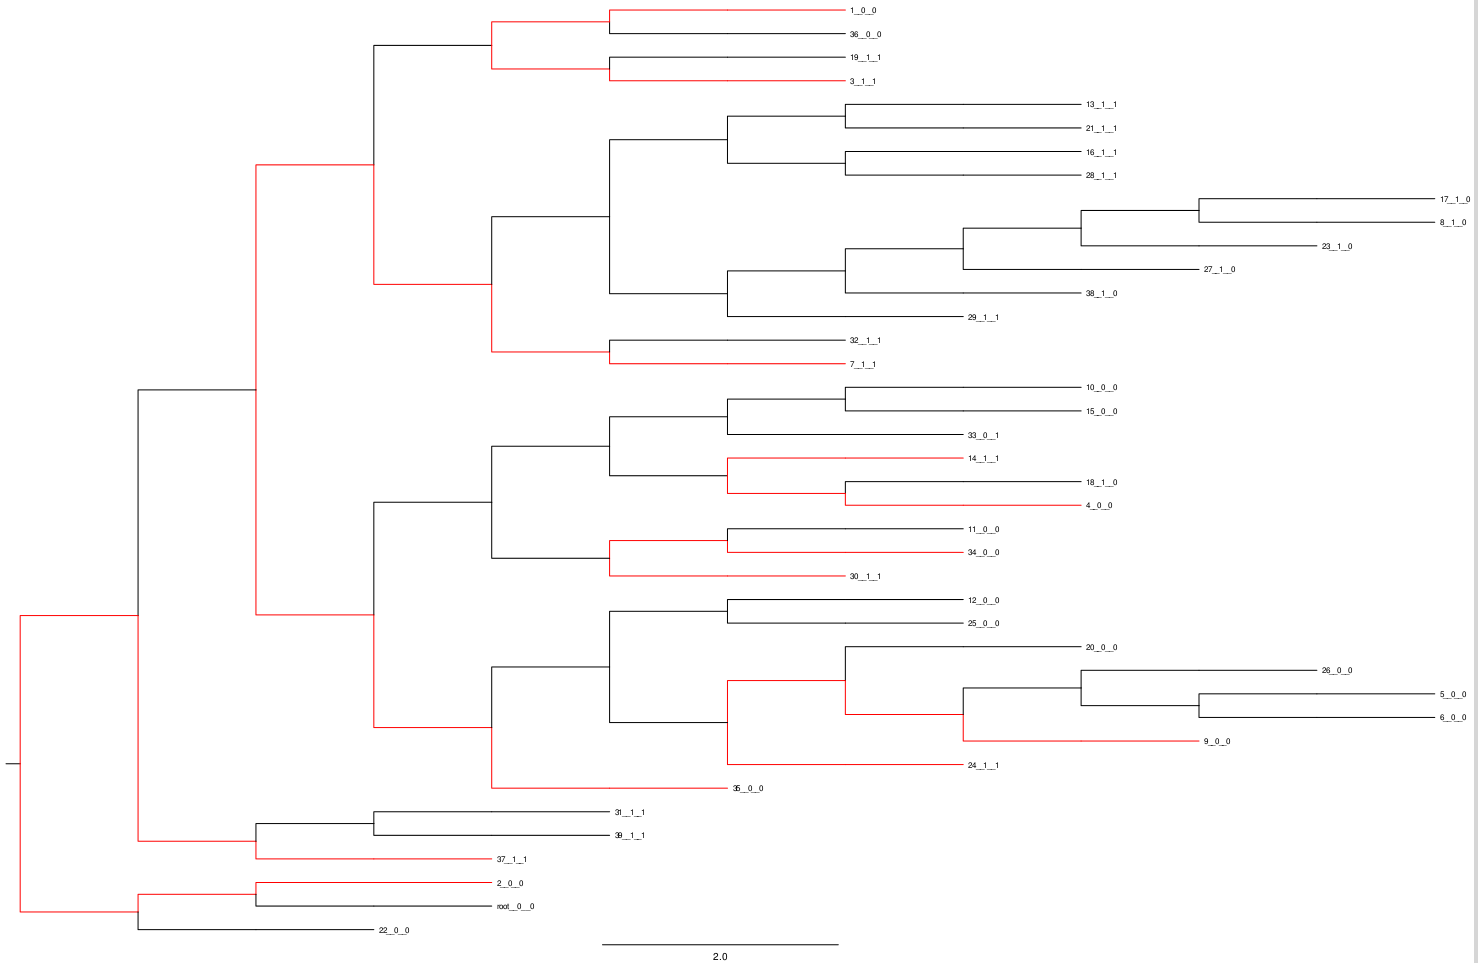
\includegraphics[width=\linewidth]{images/bestpossible.png}
      \caption{A best possible pairing}
      \label{fig:best}
    \end{figure}

    The tree in Figure \ref{fig:best} has a maximum of 6 contrasting pairs, and in this tree the pairs have been chosen so that all pairs support \verb+A->B+. (The presence of the gene caused the presence of the phenotype). However, in this particular tree we could also have picked 6 contrasting pairs where not all pairs supports this. See for example the pairing in Figure \ref{fig:worst}: \\

    \begin{figure}
      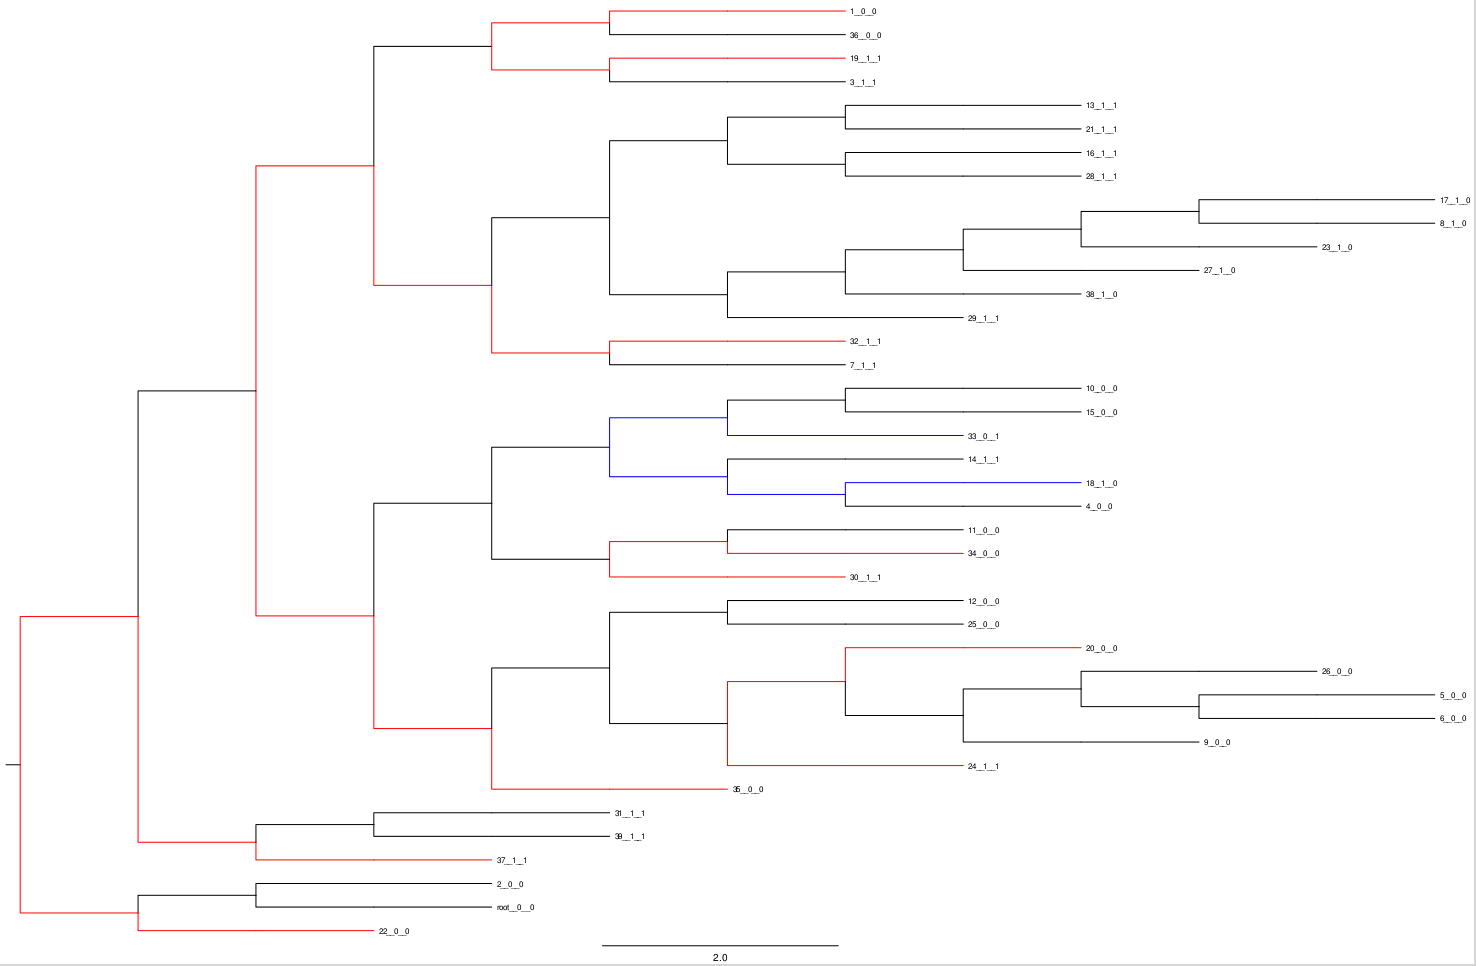
\includegraphics[width=\linewidth]{images/worstpossible.png}
      \caption{A worst possible pairing}
      \label{fig:worst}
    \end{figure}

    The tree in Figure \ref{fig:worst} has the same topology and terminal states, and the same number of contrasting pairs, but now we have chosen pairs so that 5 pairs support \verb+A->B+ while 1 pair oppose it (It suggests that \verb+A->b+/ \verb+a->B+). This is a worst possible pairing which maintains the maximum number of contrasting pairs. \\

    Scoary reports the best (lowest) and worst (highest) p-values, corresponding to the first and the second scenario, respectively. The p-value corresponds to a binomial test using the number of supporting pairs as successes and a probability of 0.5 for each state. A $p<0.05$ would thus typically be considered as a rejection of the null hypothesis that the expressed phenotype is not associated with the gene. \\

  \section{Example data}
    In the exampledata folder you can see an example of how the input files would typically look. This simulated and completely fictitious data set consists of 100 isolates with around 3000 core genes and a total pan-genome of around 9000 genes. \\ 

    Here I have used tetracycline resistance as the phenotype for which we would like to know the genetic basis. In this example, only a single gene controls the expression of tetracycline resistance, although the penetrance of the gene is not 100\% (i.e. isolates can have the gene and still be susceptible towards tetracycline), and other, unmeasured factors (for example point mutations) can also induce resistance. \\

    For demonstration purposes I have also included a second phenotype, called Bogus, which has been generated completely at random, and so doesn't have any association to any of the genes in the gene presence/absence file. \\

    This particular example very clearly identifies the causal gene (looking at the pairwise comparison p-values), whereas in real experiments the results are sometimes a lot messier. \\

    Running Scoary with the --test flag is equivalent to the following command: \\
    \begin{lstlisting}[language=python, basicstyle=\small]
      $ scoary -t ./exampledata/Tetracycline_resistance.csv -g ./exampledata/Gene_presence_absence.csv -u -c I EPW
    \end{lstlisting}

  \section{Example use cases}
    Below are presented some popular use cases with examples of how to run and interpret results. \\

    \textbf{1. Resistance towards an antibiotic compund in Mycobacterium abscessus} \\
    A user wanted to screen for possible genetic causes of resistance towards a new antibiotic in Mycobacterium abscessus. One hypothesis was that the resistance could be related to a truncated form of a gene. In this experiment, the user had classified the resistance pattern as (S)usceptible, (I)ntermediate and (R)esistant. This information was coded into the traits file as dummy variables, e.g. the first trait was SI\textunderscore vs\textunderscore R and the second was S\textunderscore vs\textunderscore IR. \\

    Mycobacterium abscessus contains numerous subspecies, and the user wanted to test only M. abscessus ss abscessus. The Roary output additionally contained other subspecies, such as M. abscessus ss masiliense. To avoid altering the Roary file, a csv was made containing the names of all isolates that were M. abscessus ss abscessus. To write a separate gene presence/absence file from only these isolates (and to speed up analysis), the -w parameter was used. \\

    A high number of isolates was used in the experiment, and it was therefore decided to set the significance threshold high (i.e. require low p-values). The experiment was interested in causal mutations, so pairwise comparisons had to be used. (Population structure could be a major confounder). It was decided to require that the entire range of pairwise comparison values should be < 1E-4. Additionally, after 10.000 permutations the input configuration should be in the top 0.1 percentile. (Among 10.000 randomly permuted datasets, no more than 9 were allowed to have a even higher number of contrasting pairs for a gene to be included in results). \\

    A ML phylogeny was built with a dedicated tree program and provided as a custom tree. \\

    Finally, since it was possible that the resistance determinant was inherited as a set of genes (such as a plasmid), the --collapse flag was used to collapse genes with identical distribution patterns. \\

    The analysis was run with the following command: \\
    \begin{lstlisting}[language=python, basicstyle=\small]
      $ scoary -t Resistancefile -g Gene_presence_absence.csv -p 1E-4 1E-3 -c EPW P -e 10000 -w -r OnlyAbscessusIsolates.csv --collapse -n raxmltree.nwk
    \end{lstlisting}

    Results showed that the top two hits were different alleles of the same gene, one positively and one negatively associated with the trait. (The two alleles were different enough to not be clustered as the same by Roary). The interpretation was that this gene was likely to play a role in the resistance pattern. \\

    \textbf{2. Enrichment of genes in select host groups} \\

    Another user had a high number of E. coli isolated from different hosts, and wanted to know which genes were enriched in which host groups. In this case, Scoary was not used to infer causal association, but simply to discover trends in different sets. The input trait file consisted of dummy variable memberships to different host groups, reminiscent of the below table: \\
    
    \LTXtable{\textwidth}{tables/t3.tex}

    Here, the user is not trying to infer which genes "cause" membership in a group, just which genes are overrepresented. Therefore, the --no\textunderscore pairwise flag was used. The Benjamini-Hochberg adjusted p-value was used to only show the genes most overrepresented in a specific host group. \\

    The analysis was run with the following command: \\
    \begin{lstlisting}[language=python, basicstyle=\small]
      $ scoary -g gene_presence_absence.csv -t Hostgroup_membership.csv -p 1E-5 -c BH --no_pairwise
    \end{lstlisting}

    \textbf{3. SNPs linked to penicillin resistance in Neisseria meningitidis} \\

    For population structure-aware association analysis to work, it is imperative to work on trees that best represent the genealogy of the input sample. Due to the high frequency of recombination in Neisseria meningitidis, the internal tree builder in Scoary is likely to perform poorly. In this case (actually, in almost any case) it would be advisable to use a dedicated tree program and provide this to Scoary instead. There are now many programs that can produce phylogenetic trees where only the clonally evolved patterns are retained (i.e. "free" from the obfuscating effects of recombination). Some examples are Gubbins, ClonalFrameML and BRATNextGen. \\
    
    \begin{lstlisting}[language=python, basicstyle=\small]
      $ scoary -g gene_presence_absence.csv -t penicillinres.csv -n clonaltree.nwk
    \end{lstlisting}

  \section{License}
    Scoary is freely available under a GPLv3 license. \\

  \section{Etymology}
    Scoary is an anagram of "scoring" and "Roary", the pan-genome pipeline. It was named as an homage to Roary. \\

  \section{FAQ}
    \textbf{How can you justify p=0.5 in your pairwise comparisons method? Is this species-specific?} \\

    The reasoning is as follows: Scoary first finds the maximum number of independent contrasting pairs in a phylogenetic tree, irrespective of gene-trait status. Thus, AB-ab pairs should be equally likely as Ab-aB pairs if your null hypothesis is true. Your null hypothesis in this case, is that there is no detectable association between A/a and B/b. If AB-ab pairs are much more common than Ab-aB pairs then you can be confident that the true p was not 0.5. And if this is the case then then there seems to be an association between your A/a (your gene) and your B/b (your phenotype). Further details can be found in Read and Nee, 1995. \\
    
    \textbf{Why is my "Best\textunderscore pairwise\textunderscore comp\textunderscore p" higher than my "Worst\textunderscore pairwise\textunderscore comp\textunderscore p"? (No longer relevant in version 1.6.x)}\\

    The "best" and "worst" labels are attached to the odds ratio of the gene in the non-population structure-corrected analysis. For example, you may find an odds ratio of 2.0 for a particular gene, meaning presence of the gene was tied to presence of the phenotype. But when you inspect your pairwise comparisons p-values you see that the "best" p-value was 0.2 and the "worst" was $1.0E-5$. This means that in your phylogenetic tree, an enrichment of Ab-aB pairs was more common. In other words, the presence of this gene actually seems associated to a \textit{silencing} of the phenotype, in spite of your original odds ratio. Note that the odds ratio can be inflated for example by sampling of very closely related isolates. \\
    
    \textbf{Can I use this for SNPs/kmers?} \\

    In theory yes, but it requires some tinkering. Obviously you couldn't take the input file directly from Roary. You'd have to create the input file yourself. In theory, this shouldn't be too hard. Just have each row be a single SNP/kmer rather than a gene. Note that each variant has to be binary, so if you have SNPs with three (or more) alleles this complicates interpretations, particularly if they have differential effect on the outcome. \\
    
    \textbf{A lot of my empirical p-values are identical. Bug?} \\

    Not really. In order to save time, Scoary calculates the empirical p-values as it goes through permutations. If it sees early on that a particular variant is not interesting (e.g. empirical p-value above 0.1) it does not waste any more resources on this variant. As a result, note that higher empirical p-values are less accurate (because they have been calculated from fewer permutations). \\
    
    \textbf{Do I need to convert my gene\textunderscore presence\textunderscore absence.csv file into 1s and 0s rather than gene/locus\textunderscore tag names?} \\

    No. Scoary treats "0", "-" and "" as gene absence, anything else as presence. You should be able to feed the file directly from Roary. \\
    
    \textbf{Can I use this for archea?} \\

    Honestly, I don't know enough about archea to say for sure. \\
    
    \textbf{Can I use this for human/mouse/plant/fungus?} \\

    Most certainly not. \\

  \section{Acknowledgements}
    \begin{itemize}
      \item Marco Galardini cleaned my code and made many nifty improvements.
      \item Anders Goncalves da Silva made Scoary installable by pip
      \item The QuadTree and UPGMA implementation was heavily based on code by Christian Storm Pedersen.
      \item Ines Mendes pointed out a number of bugs related adjusted p-values and isolate restriction.
      \item Eric Deveaud added versioning.
    \end{itemize}

  \section{Feedback}
    I greatly appreciate any feedback, even negative. If you like (or dislike) Scoary, please feel free to tell your friends and colleagues about it. If you don't have friends or colleagues, please feel free to rant about it on your blog or social media profile. \\

  \section{Citation}
    If you use Scoary, please consider citing: \\
    
    \textbf{Brynildsrud O, Bohlin J, Scheffer L, Eldholm V.} Rapid scoring of genes in microbial pan-genome-wide association studies with Scoary. \textit{Genome Biol.} 2016;17:238 \\

    The article is Open Access, and can be found using DOI: 10.1186/s13059-016-1108-8 \\

  \section{Contact}
    Ola Brynildsrud (ola.brynildsrud@fhi.no) \\

  \bibliography{citations}
  \bibliographystyle{unsrt}

\end{document}